\begin{frame}[fragile]{Architettura}
	\begin{figure}[h] 
		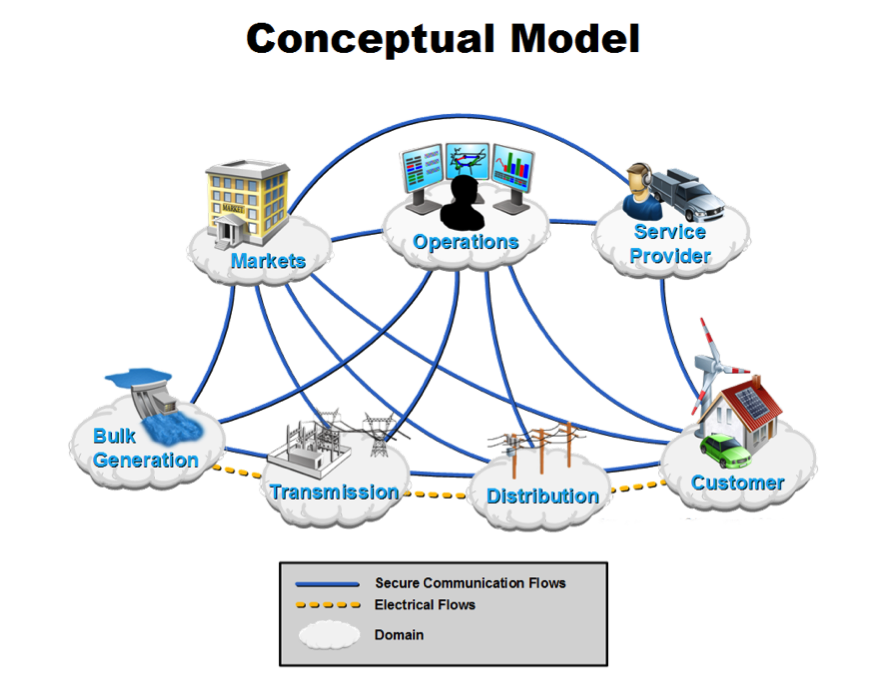
\includegraphics[scale=0.6]{imgs/sg.png}
	\end{figure}
\end{frame}

% Energy and supporting ancillary services (capacity that can be dispatched when needed) are procured through the Markets domain, scheduled and operated from the Operations domain, and finally delivered through the Transmission domain to the distribution system and finally to the Customer domain.

\begin{frame}[fragile]{Architettura}
	\vspace{-10pt}
	\begin{figure}[h] 
		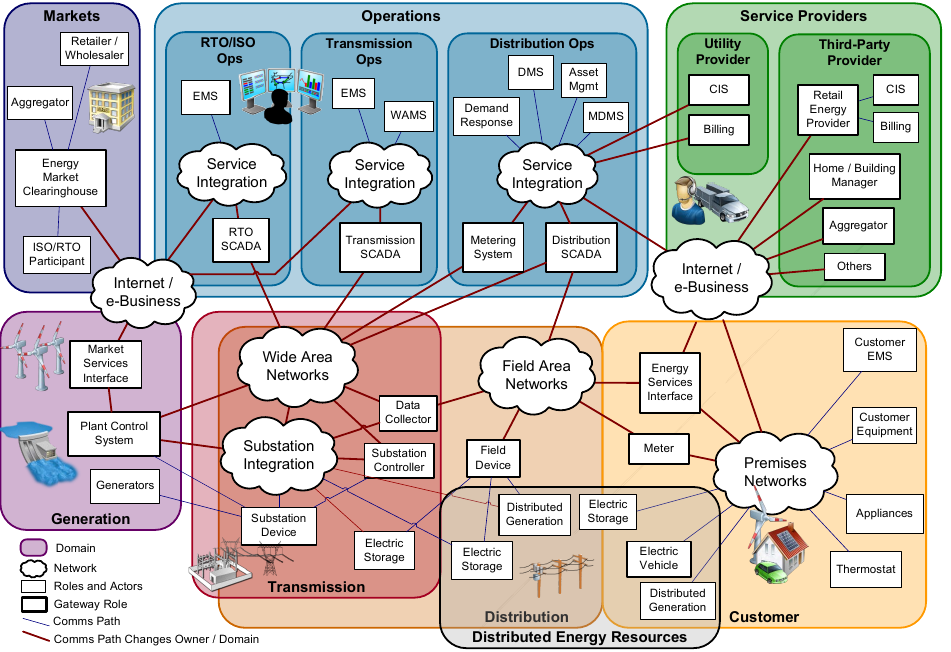
\includegraphics[scale=0.45]{imgs/arch.png}
	\end{figure}
\end{frame}

%\begin{frame}[fragile]
%  \frametitle{Smart Grid Framework}
%	\begin{figure}[h] 
%		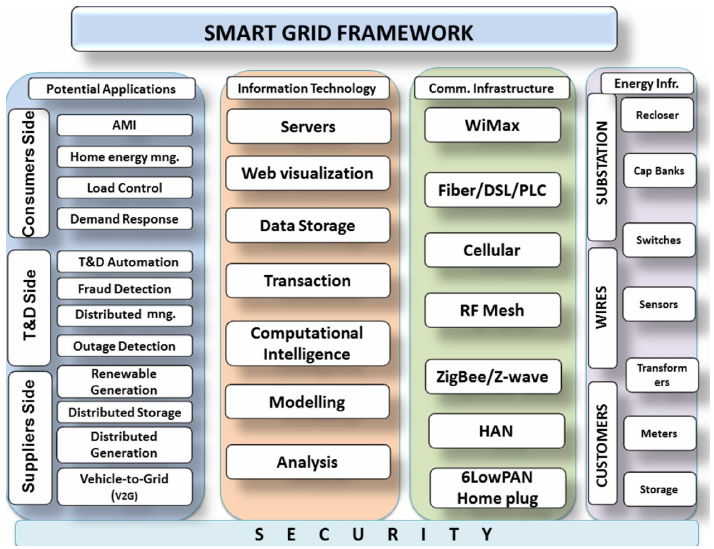
\includegraphics[scale=0.6]{imgs/sgframework.png}
%	\end{figure}
%\end{frame}

%%% CUSTOMER %%% 

\begin{frame}[fragile]{Customer} 
	\begin{figure}[h] 
		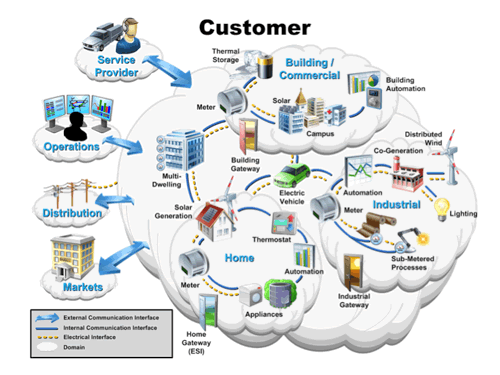
\includegraphics[scale=0.45]{imgs/cust.png}
	\end{figure}
\end{frame}

\begin{frame}[fragile]{Customer} 
		\begin{block}{Smart meter}
		 E' un dispositivo elettronico che registra consumi di energia elettrica
		\begin{itemize}
			\item Comunica informazioni per scopi di fatturazione
			\item Blocca la fornitura di energia  % bad pay o demande response
			\item Notifica informazioni per monitoraggio e in caso di manomissione % comunica con i display   
		\end{itemize}
		\end{block}
		\pause
		\begin{block}{Advanced Metering Infrastructure} % sistema che integra smart meter, display, termostati ecc., reti di comunicazione verso i concentratori di dati e sistemi di gestione dei dati
		\begin{itemize}
			\item Consente una comunicazione bidirezionale fra utility e consumer % ciò consente di inviare comandi per info di pricing basate sul tempo, azioni di domanda risposta o disconnessioni remote
			\item Misura, colleziona, analizza il consumo energetico e comunica con smart device
		\end{itemize}		
		\end{block}	
\end{frame}

%%% MARKETS %%% 

% I mercati sono il luogo in cui le attività di rete vengono acquistate e vendute
% La comunicazione tra il dominio dei mercati e dei domini che forniscono energia sono fondamentali per una efficiente corrispondenza  di produzione con il consumo è dipendente dai mercati. I domini di approvvigionamento energetico sono il dominio di Bulk gen e delle Risorse energetiche distribuite (DER)
% Comunicazioni per le interazioni di dominio dei mercati devono essere affidabili. Essi devono essere tracciabili e verificabili.
\begin{frame}[fragile]{Markets}
	\begin{figure}[h] 
		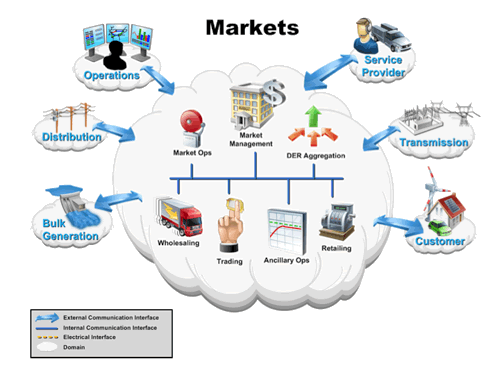
\includegraphics[scale=0.45]{imgs/market.png}
	\end{figure}
\end{frame}

%%% SERVICE PROVIDER %%%

% supporta i processi di business dei produttori del sistema di alimentazione, distributori e clienti
% Questi processi di business vanno da servizi di pubblica utilità tradizionali, come la gestione della fatturazione e conto del cliente, ai servizi avanzati al cliente, come la gestione del consumo energetico e la produzione di energia casalinga.
\begin{frame}[fragile]{Service Provider}
	\begin{figure}[h] 
		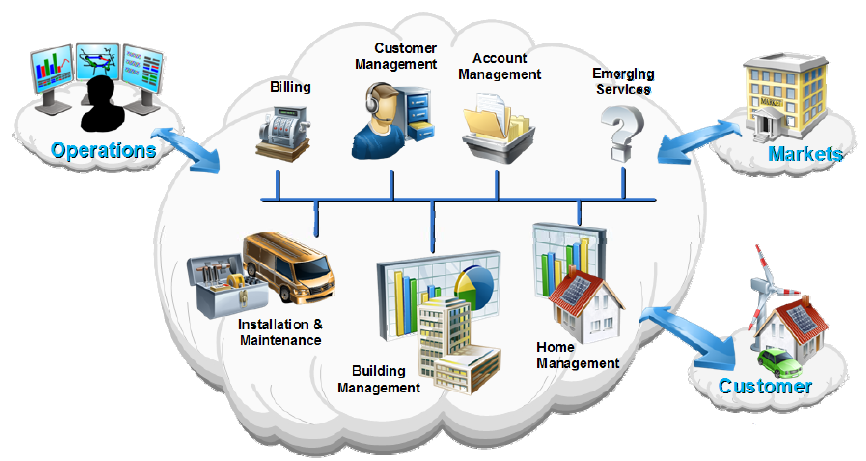
\includegraphics[scale=0.45]{imgs/ser.png}
	\end{figure}
\end{frame}

\begin{frame}[fragile]{Service Provider}
	\begin{itemize}[<+- | alert@+>]
		\item Sviluppano interfacce e standard per un sistema basato su un modello di mercato dinamico, proteggendo le infrastrutture di energia critiche   
		\item Non devono compromettere la sicurezza informatica, l'affidabilità, la stabilità, l'integrità o la sicurezza della rete %quando forniscono servizi esistenti o emergenti
		\item Creano servizi e prodotti per rispondere alle nuove esigenze e le opportunità offerte dall'evoluzione delle Smart Grid 
		\item Rappresentano una zona di notevole nuova crescita economica
	\end{itemize}
\end{frame}



%%% OPERATION %%% 

% responsabile del buon funzionamento del sistema di alimentazione.
\begin{frame}[fragile]{Operations}
	\begin{figure}[h] 
		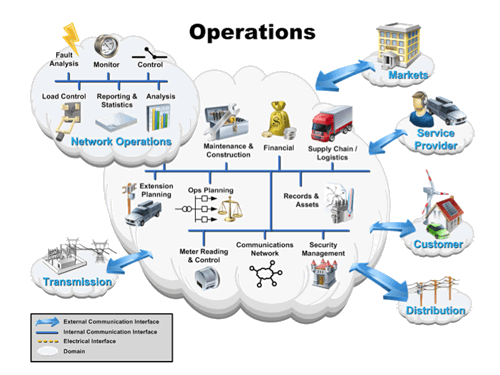
\includegraphics[scale=0.45]{imgs/ope.png}
	\end{figure}
\end{frame}

% Monitoring: supervisionare la topologia della rete, connettività, condizioni di carico, include i dispositivi intelligenti (IED) e dispositivi sul campo, in grado di reportare lo stato della rete

% Control: supervisiona ampie aree, substation, controlli automati o manuali

% Fault Management: migliora la velocità di identificazione di fault, in modo da effetturare ripristino

% Analysis: si confrontano dati in tempo reale e non per ricavare info su incidenti di rete, connettività per scopi di manutenzione

% Operational Planning: mantengono il costo basso della potenza attraverso la generazione di picco, la commutazione, eliminazione del carico o la risposta alla domanda.



%%% GENERATION %%%

% Fornisce energia ai consumers. La generazione di energia è il processo di creazione di energia da diverse fonti energetiche. Tale energia viene portata attraverso il sistema di trasmissione. Comunicazioni con il dominio di trasmissione sono le più critici perché senza trasmissione, i clienti non possono essere serviti.
\begin{frame}[fragile]{Generation}
	\begin{figure}[h] 
		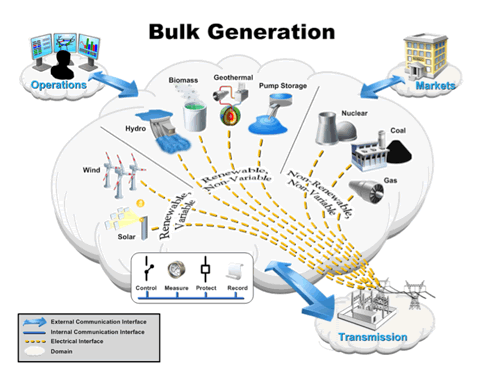
\includegraphics[scale=0.45]{imgs/gen.png}
	\end{figure}
\end{frame}

\begin{frame}[fragile]{Generation}
	\begin{itemize}[<+- | alert@+>]
		\item Gestire il flusso energetico e l'affidabilità del sistema % fasori su substation per modificarne il flusso
		\item Reagire rapidamente ai guasti, interruzioni di corrente o abbassamenti di tensioni % per alta affidabilità
		\item Monitoraggio delle strutture per valutarne le condizioni
		%\item Cruciali risultano comunicazioni in caso di guasti o scarsa fornitura d'energia % energy storage presente su sistemi di trasmissione e distribuzione devono aiutare
	\end{itemize}
\end{frame}


%%% TRASMISSION %%% 

% Trasferimento di massa di energia elettrica da fonti di generazione alla distribuzione attraverso molteplici substation
% include remote terminal units, substation meters, protection relays, power quality monitors, phasor measurement units, sag monitors, fault recorders, e substation user interfaces.
\begin{frame}[fragile]{Transmission}
	\begin{figure}[h] 
		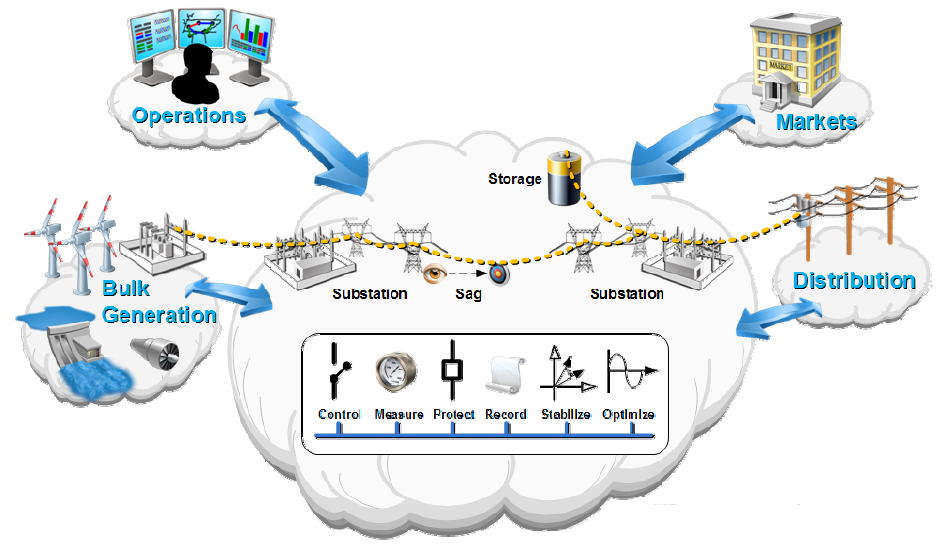
\includegraphics[scale=0.45]{imgs/tras.png}
	\end{figure}
\end{frame}

% rilevatore di abbassamento di linea (sag)
\begin{frame}[fragile]{Transmission}
	\begin{itemize}[<+- | alert@+>]
		\item Gestita da un Regional Transmission Operator o Independent System Operator (RTO/ISO)
			\begin{itemize}
				\item Mantiene la stabilità della rete bilanciando la generazione con la domanda energitica
			\end{itemize}				
		\item Monitorata da sistemi di supervisione e controllo di acquisizione dati
		\item Composta da substation, torri di trasmissione, linee elettriche e dispositivi di telemetria	 
	\end{itemize}
\end{frame}

% Una substation elettrica è un punto di riferimento dei sistemi di generazione, trasmissione e distribuzione, dove il voltaggio viene trasformato da alto a basso e viceversa mediante trasformatori. Ci sono diversi tipi di substation: trasmissione, distribuzione, raccolta, smistamento.
\begin{frame}[fragile]{Transmission}
	\begin{itemize}[<+- | alert@+>]
		\item Le substation sono una componente chiave del sistema di trasmissione
		\begin{itemize}
			\item 
		\end{itemize}
	\end{itemize}
\end{frame}
%%% DISTRIBUTION %%% 

\begin{frame}[fragile]{Distribution}
	\begin{figure}[h] 
		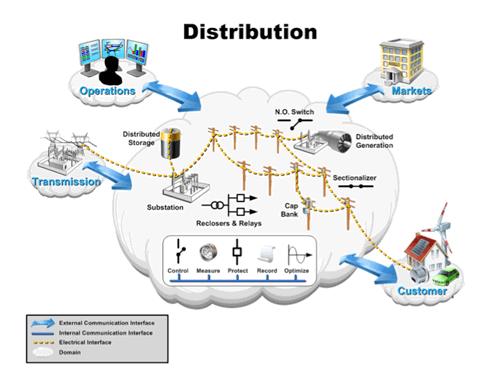
\includegraphics[scale=0.45]{imgs/distr.png}
	\end{figure}
\end{frame}
